\documentclass{report}

% import template created by SeniorMars
\input{preamble}

\title{A Comprehensive Review of Agricultural Parcel and Boundary Delineation from Remote Sensing Images: Recent Progress and Future Perspectives}
\author{Juepeng Zheng et al.}
\date{}

\usepackage[backend=biber, style=authoryear, style=numeric, sorting=none]{biblatex}  % citations
\addbibresource{references.bib}                         % references file
\usepackage[font=small, textfont=bf]{caption}           % dont enumerate image captions
\usepackage{csquotes}                                   % for styled quotes
\usepackage{float}
\usepackage{graphicx}                                   % to import images
\graphicspath{{./images/}}                              % images dir
\usepackage{parskip}                                    % start paras on new lines instead of with indents

% match section ordering style with paper wherever possible
\renewcommand{\thesubsection}{\Roman{subsection}}
\setcounter{secnumdepth}{3} % ensure subsubsections are numbered (default is usually 3)
\renewcommand{\thesubsubsection}{\Alph{subsubsection}} % use alphabets for ordering subsubsections

\begin{document}

\maketitle
\tableofcontents

\chapter{Research Summary}

% preface
\begin{center}
  \small
  \textbf{Preface} \\
  \vspace{1em}
  This report provides a comprehensive summary and critical analysis of 
  \citetitle{zheng2025comprehensivereviewagriculturalparcel} by \citeauthor{zheng2025comprehensivereviewagriculturalparcel} 
  The following sections synthesize the 
  authors' framework, methodology, and key findings regarding Agricultural 
  Parcel and Boundary Delineation (APBD)
  \vspace{1em}
\end{center}

\section{Introduction}

\dfn{Agricultural Parcel and Boundary Delineation}{
  \textbf{Agricultural Parcels} represent the fundamental spatial units for agricultural activity.
  \newline

  \textbf{Agricultural Parcel and Boundary Delineation (APBD)} is an interdisciplinary application of computer
  algorithms for vision tasks where agricultural fields are disected into their component parcels, and 
  distinctly separated from their background (adjacent parcels, natural vegetation and other types of land).
}

Applications of APBD include:
\begin{itemize}
  \item sustainable agriculture planning and land-use monitoring
  \item crop mapping
  \item yield estimation
\end{itemize}

Foundation models such as Transformer architectures, the Segment Anything Model (SAM), and Vision-Language
Vision-Language Models (VLMs), leveraging massive datasets and self-supervised learning, offer strong
generalizaton ability, high adaptability, and improved performance accross diverse agricultural
scenarios when applied to high-resolution remote sensing imagery.

The authors conceptualize APBD as composing three hierarchical levels:
\begin{enumerate}
  \item Cropland Identification
  \item Boundary Delineation 
  \item Parcel Segmentation
\end{enumerate}

The paper seeks to synthesize the emerging trends in APBD research, presenting the historical
evolution, current status, and future directions. The authors identify remote sensing data 
as a critical driver of APBD research in the foreseeable future.

\section{Meta-analysis of Related Literature}

\begin{figure}[H]
    \centering
    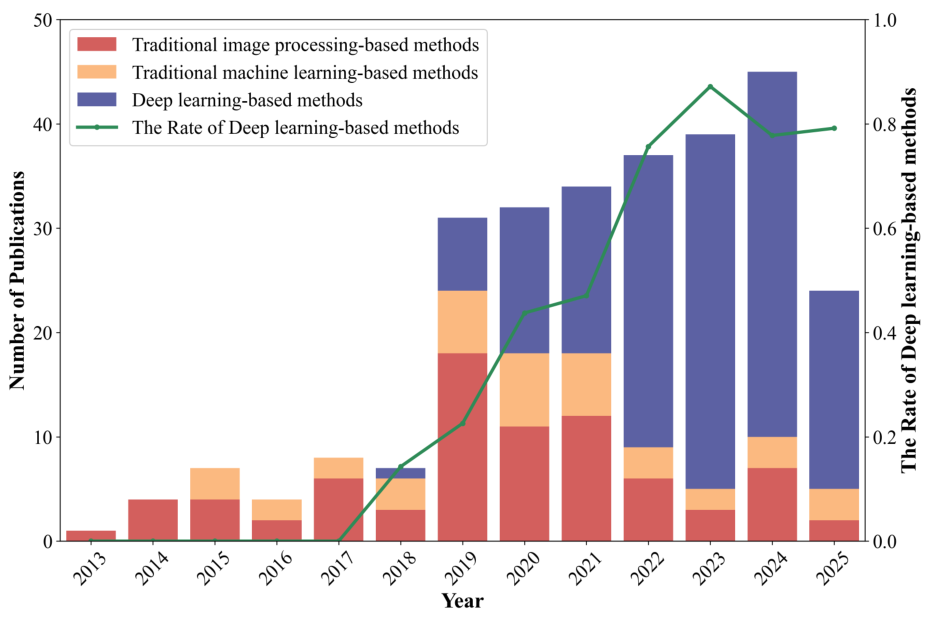
\includegraphics[width=0.7\textwidth]{fig-2}
    \caption*{Trends in APBD methodologies (Figure 2)}
\end{figure}

\subsection{Overall Trend}
\begin{itemize}
  \item \emph{\textquote{Since 2019, the number of APBD studies using Very High-Resolution (VHR) imagery has increased exponentially.}}
  \item Although VHR imagery enables high accuracy APBD, storage and processing costs prove to be a disadvantage. Large scale studies
    tend to use \textgreater 10 m spatial resolution to balance land variety and coverage, accuracy, and storage.
\end{itemize}

\begin{figure}[H]
    \centering
    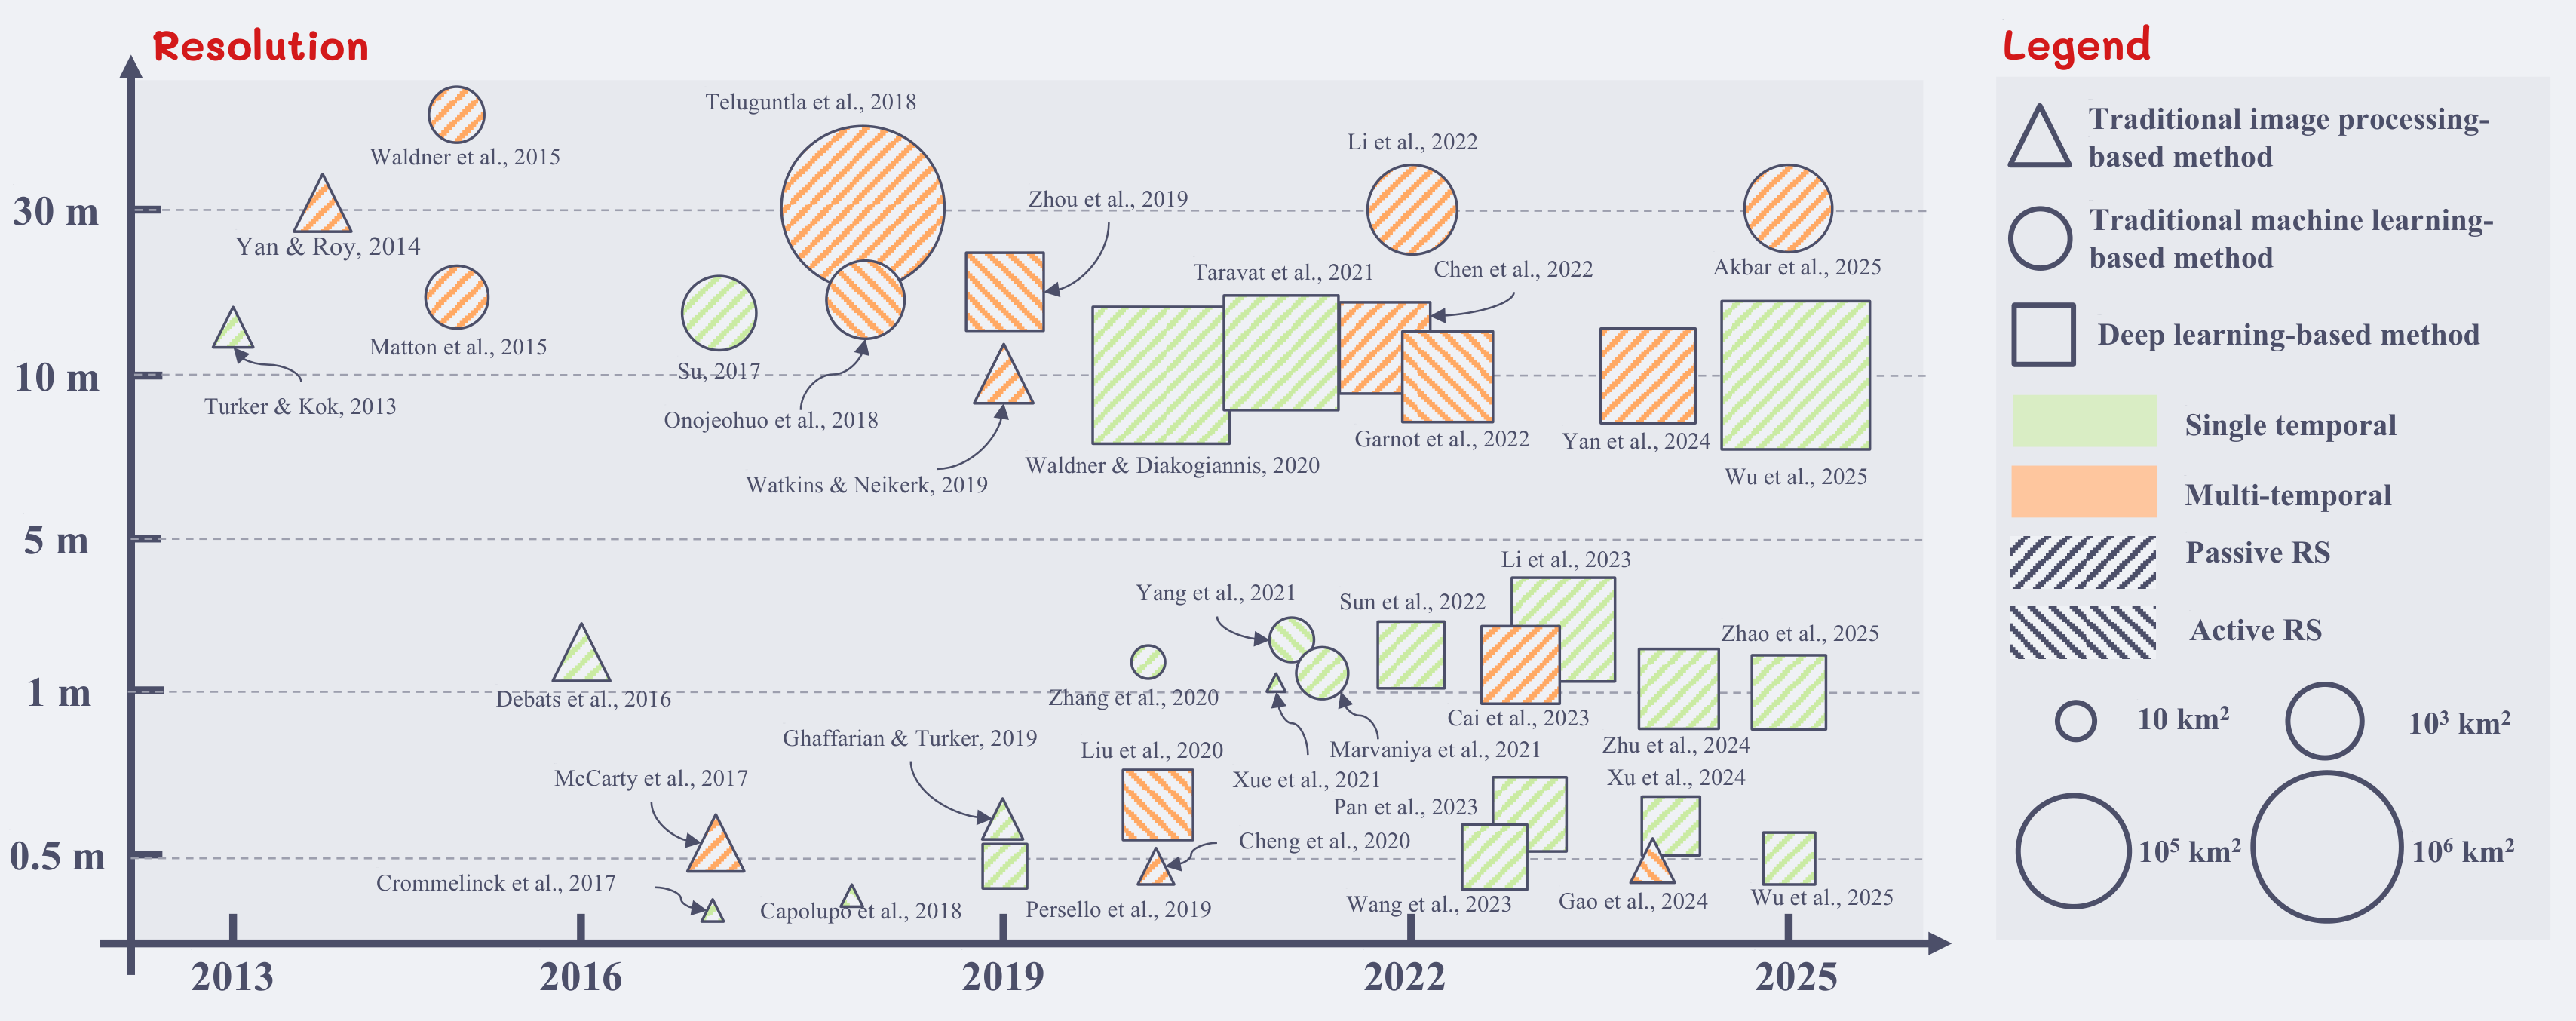
\includegraphics[width=1.0\textwidth]{fig-3}
    \caption*{Overall trends of APBD development (Figure 3)}
\end{figure}

\subsection{Quantitative Analysis}

\begin{itemize}
    \item \emph{Types of crops:} Corn crop most widely studied for APBD with statistics presented in figure 4 of the paper, attached below.

\begin{figure}[H]
    \centering
    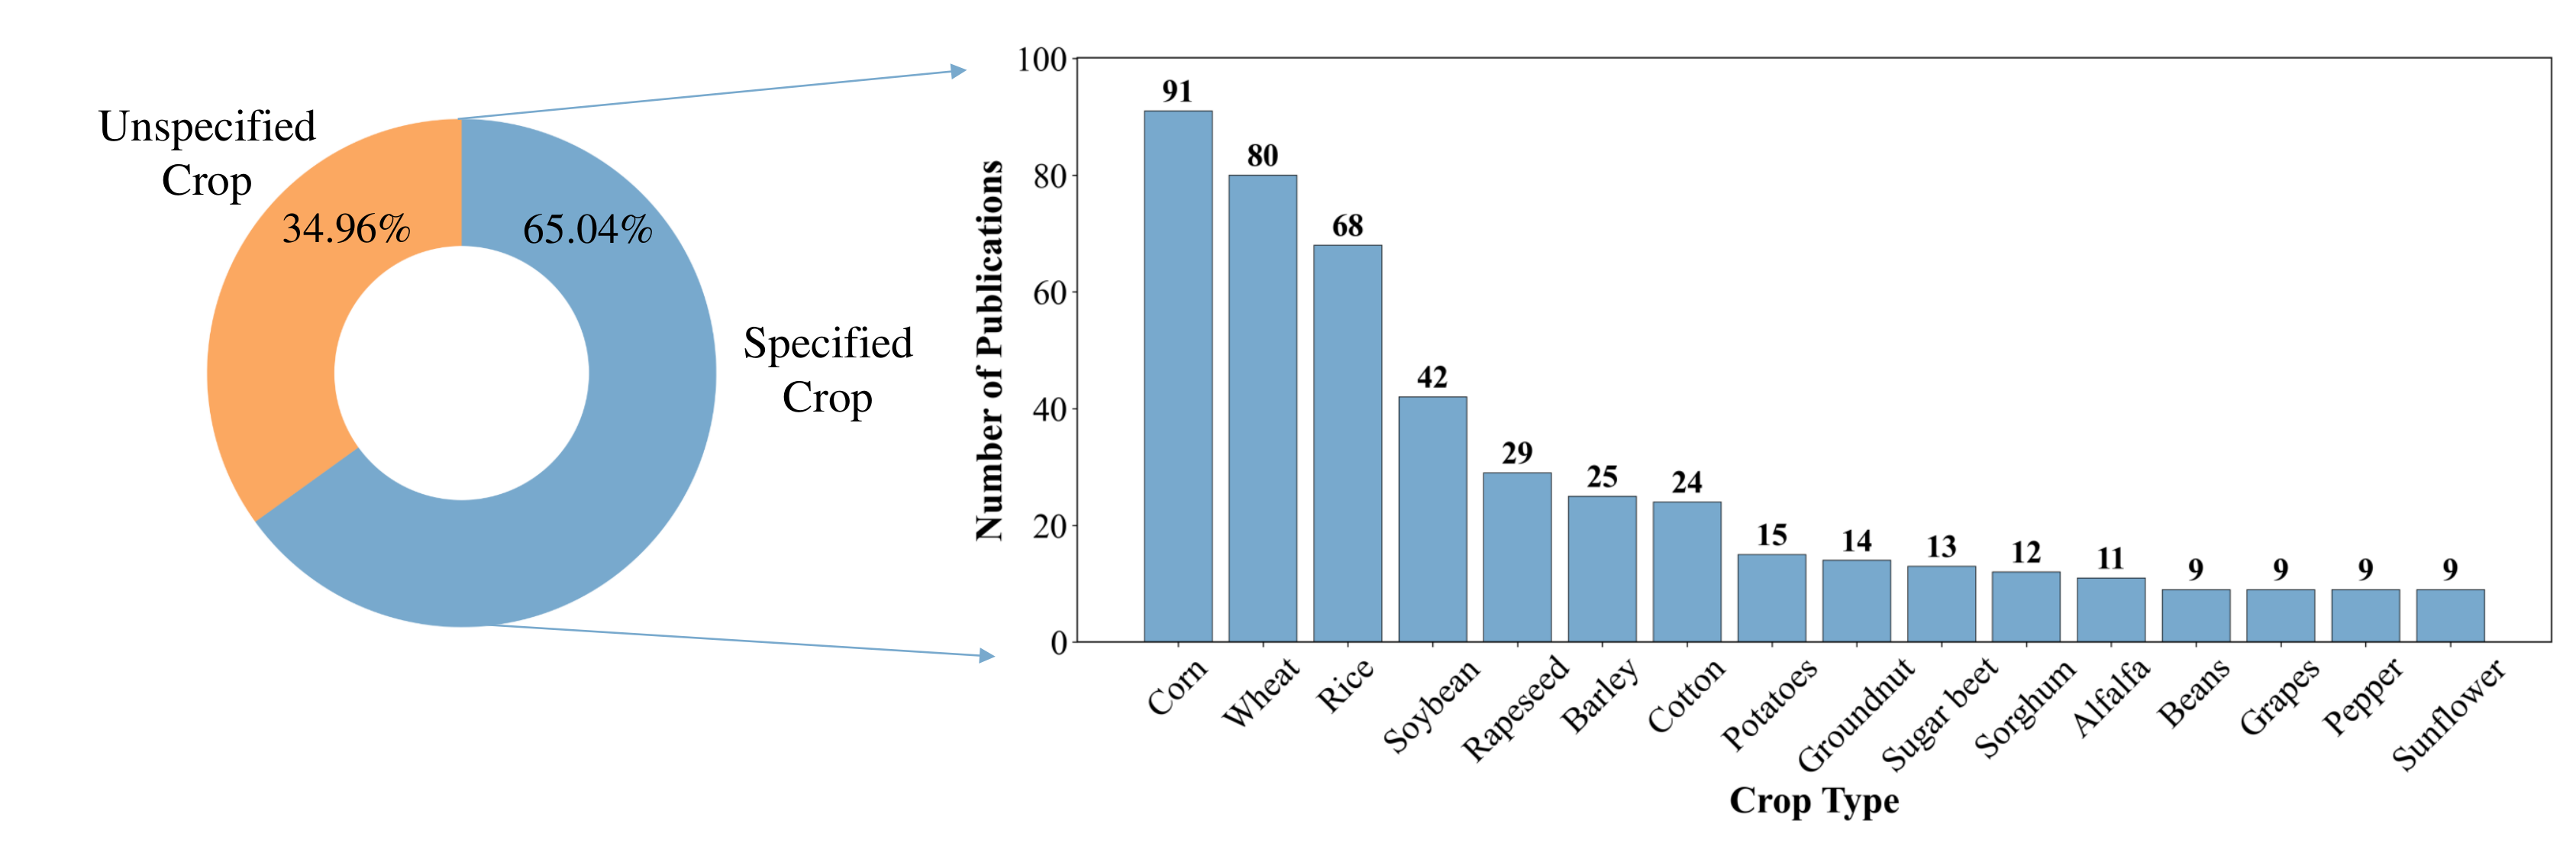
\includegraphics[width=0.7\textwidth]{fig-4}
    \caption*{Statistics of crop types in APBD-related publications (Figure 4)}
\end{figure}

    \item \emph{Study sites:} China (130 studies) leads in volume of publications followed by USA (19), Netherlands (14), and India (11).

    \item \emph{Study area:} Rising trend in extremely large region studies (\textgreater 10,000 km) catalysed by deep learning techniques.            

\begin{figure}[H]
    \centering
    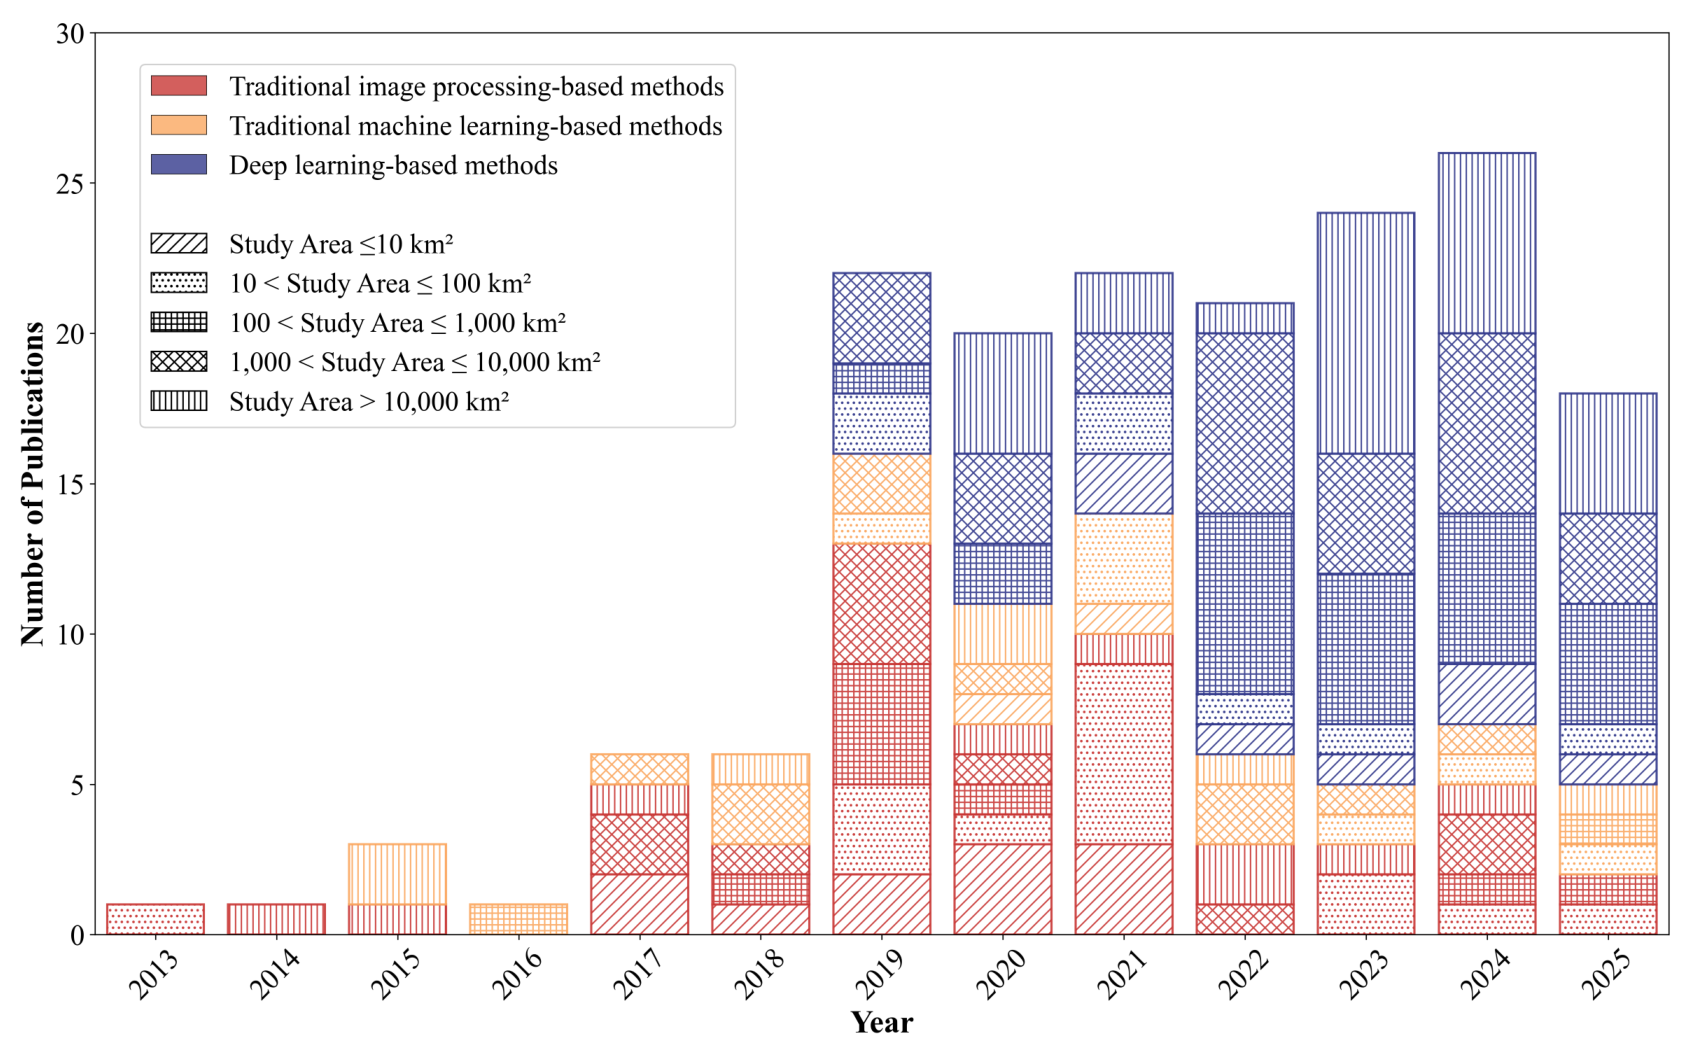
\includegraphics[width=0.7\textwidth]{fig-6}
    \caption*{Study area statistics for APBD publications (Figure 6)}
\end{figure}

\item \emph{Sensor type:} A strong reliance on satellite data (84.0\%), followed by Unmanned Aerial Vehicles (10.8\%) and aerial imagery (5.2\%).
  Sentinel (82) and Landsat (31) lead the list in medium resolution satellite imagery, while GF series (62) is the overwhelming majority in
  high-resolution ($\leq 1$m) studies.

\item \emph{Spatial resolution of data:} An increasing reliance on high-resolution imagery, attributed to the advent of modern deep learning algorithms
  that can extract detailed texture and spatial information.
\end{itemize}

\subsection{Methodology Review}
\emph{Note: for most of the algorithms and methods mentioned below, the paper provides several
good examples -- these are not covered in the summary}
\subsubsection{Traditional image processing-based methods}

Traditional methods can be classified into:

\begin{enumerate}
  \item \emph{Pixel-based methods}: Each spatially continuous unit needs to be assigned a unique label.
  \begin{itemize}
    \item \textbf{Image binaryzation} classifies pixels belonging to a parcel using thresholds. Thresholds are determined globally
      or locally - based on neighboring pixels (the latter being more robust to high-value noise and low-value boundaries)
    \item \textbf{Clustering segmentation} groups similar pixels using clustering algorithms such as k-means, fuzzy c-means, etc.
  \end{itemize}

  \item \emph{Edge-based methods}: Accurately detecting edges and boundaries between different parcels is a key challenge in APBD.
    Edge-based techniques are:
    \begin{itemize}
      \item \textbf{Traditional edge detection ("gradient") operators, such as Canny and Sobel operators,} locate
        edge of the local area by using a differential operator
        to identify locations where the gray value abruptly changes in the image
      \item \textbf{Wavelet transform} is useful for multi-resolution analysis and approximates well
        for 1-dimensional signals
      \item \textbf{Globalized Probability of Boundary (gPb)} is an advanced edge detection algorithm 
        that combines image segmentation, line detection, and contour generation integrating
        texture, color and brightness information at local and global scales
      \item \textbf{Multiscale combinatorial grouping}
      \item \textbf{Mean shift} is a nonparametric density estimation algorithm that eliminates
       the need to assume a sample distribution model and determine the number of categories,
       which can effectively reduce intra-field variation and preserve edge information
    \end{itemize}

  \item \emph{Region-based methods}: start from the inside of an object and then expand outward 
    until object boundaries are reached. 
    (assumes that neighboring pixels within the same region/parcel have similar values)
    \begin{itemize}
      \item \textbf{OBIA or GEOBIA} partitions remote-sensing imagery into meaningful image-objects
        which analyzes high spatial resolution imagery using spectral, spatial, topological, etc
        properties
      \item \textbf{Watershed segmenation} is a mathematical, morphological segmentation algorithm
        that is based on topolgy theory and simulation of the process of water immersion, but is,
        however, prone to over-segmentation.
      \item \textbf{Region growing} -- a simple and popular algorithm
      \item \textbf{Local binary fitting}

    \end{itemize}

\end{enumerate}

\begin{figure}[H]
    \centering
    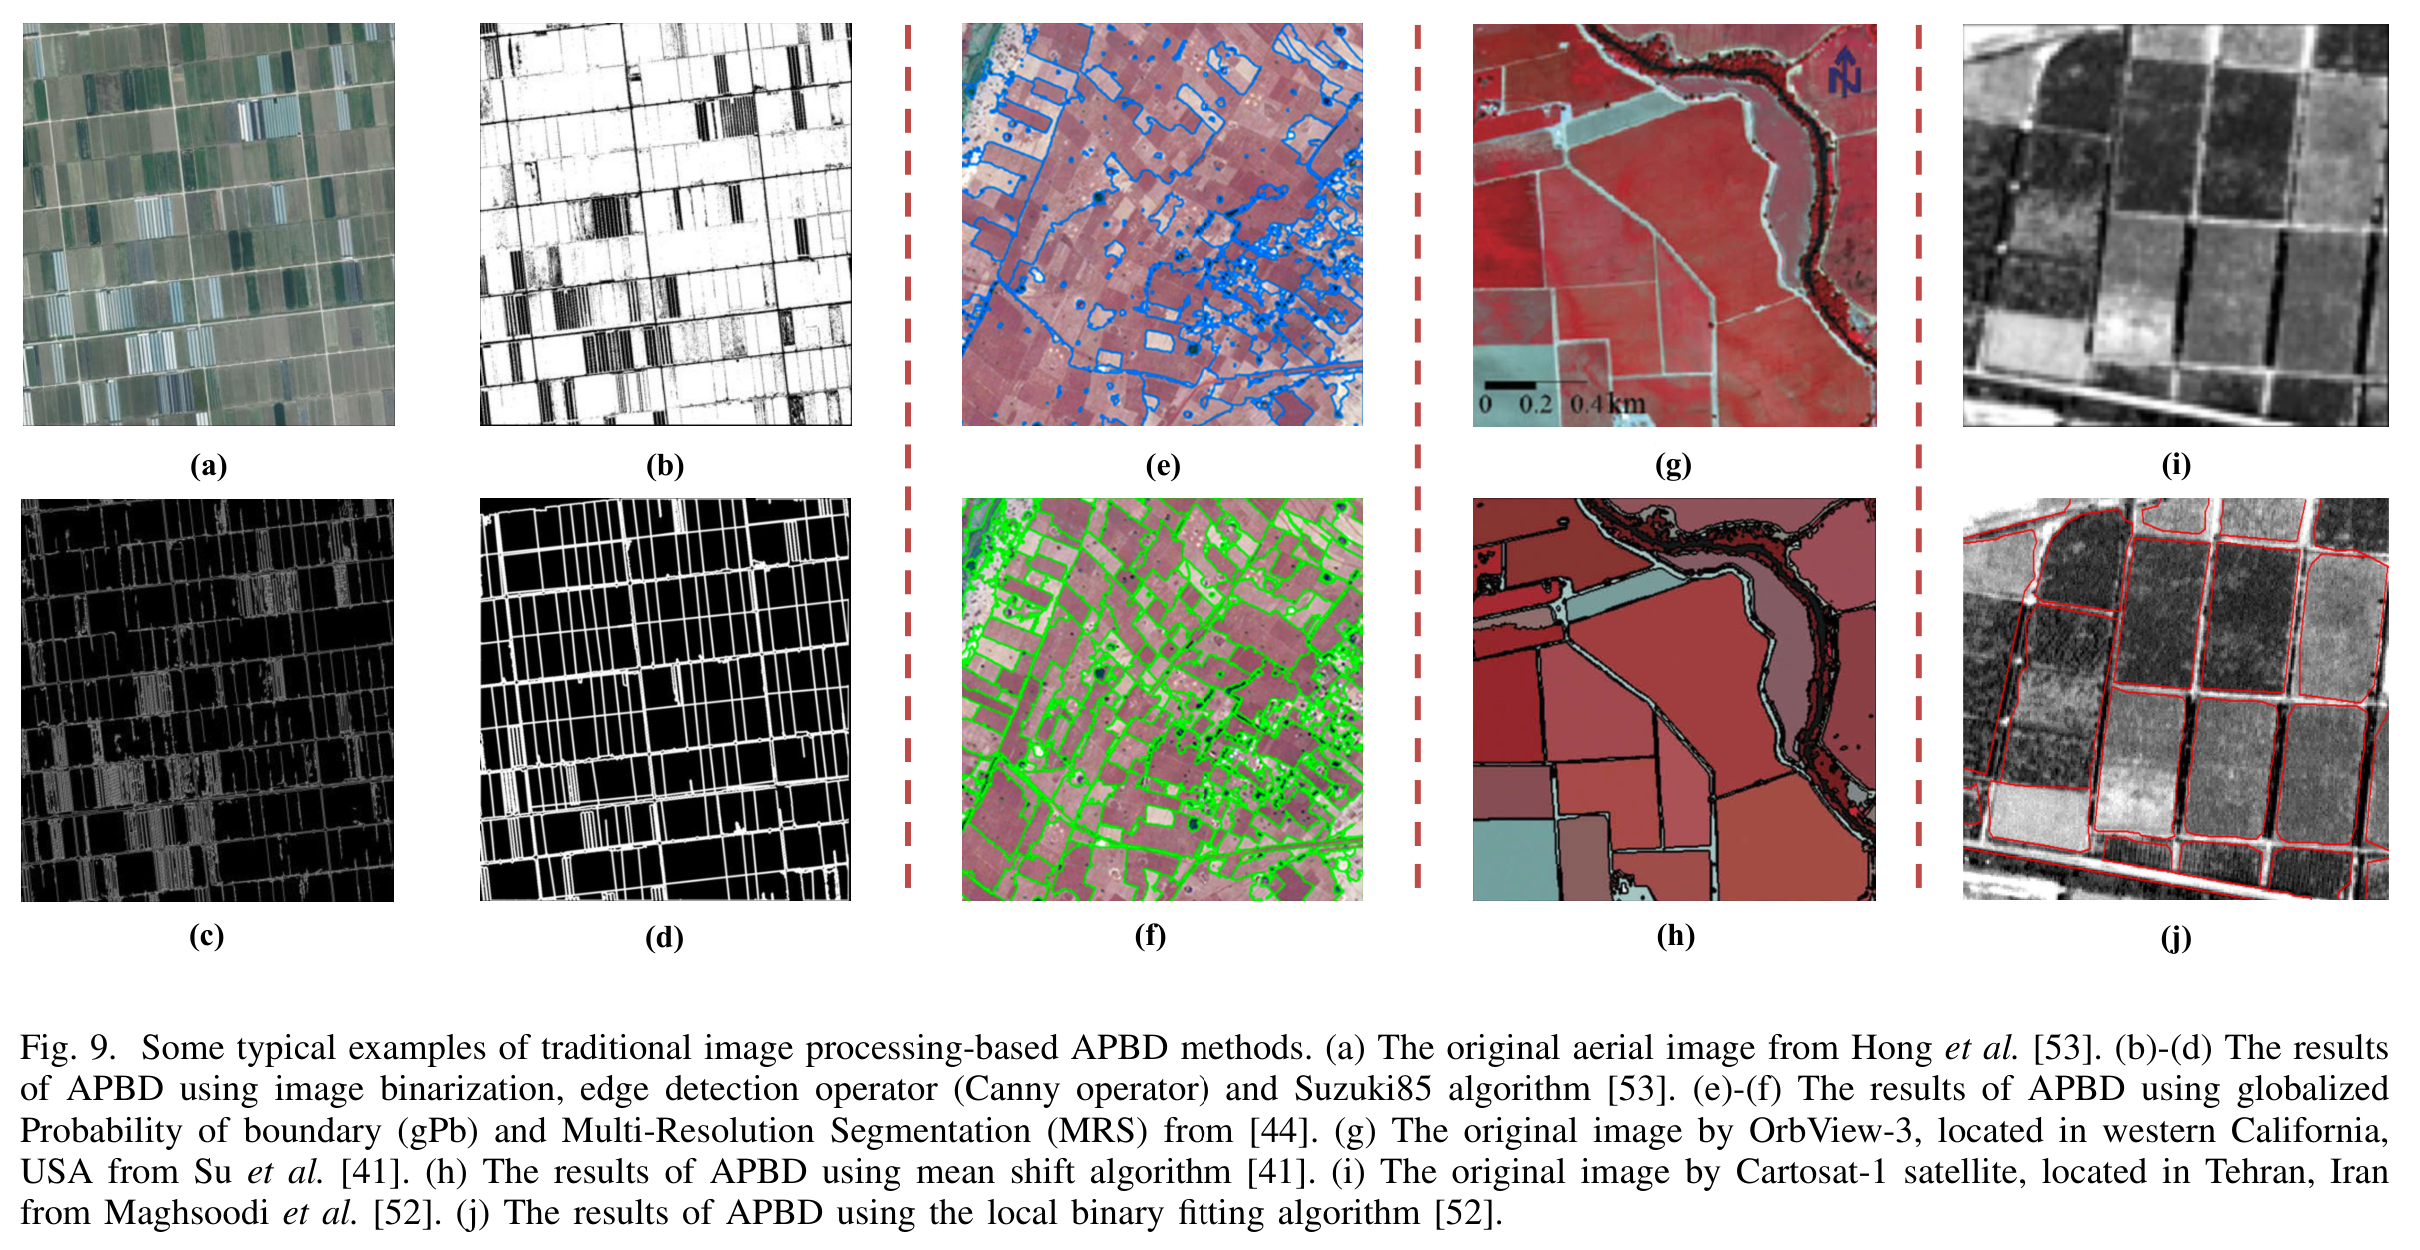
\includegraphics[width=0.9\textwidth]{fig-9}
    \caption*{Visual examples of APBD using different traditional methods (Figure 9)}
  \end{figure}

\subsubsection{Traditional machine learning-based APBD methods}
ML-based techniques are often more adpatable and generalizable than traditional deterministic methods.
The authors divide ML-based APBD into 4 steps:
\begin{enumerate}
  \item image preprocessing
  \item feature extraction
  \item classifier training
  \item model prediction
\end{enumerate}

Out of these steps, there have been different types of feature extraction and classifiers used in the task
of APBD.

\begin{enumerate}
  \item \emph{Feature extraction} includes non-handcrafted features implicit to the image such as spectral
    information, vegetation index, texture, climate characteristics, etc, as well as handcrafted features
    crafted using domain knowledge and prior context using techniques like gradient direction histogram,
    gray level co-occurence matrix, principal component analysis that capture specific visual attributes of
    parcels such as edges and shapes (helping with interpretability)
  \item \emph{Classifier training} spanning models such as Decision Trees, Gaussian maximum likelihood, SVMs,
    KNNs, logistic regression, ensemble methods, etc
\end{enumerate}

A unique approach that can enhance ML-based APBD techniques when operating on limited labels
is \emph{active learning}, where classifiers 
recognize the most informative training data based on prediction uncertainty. Estes \emph{et al.} \cite{estes2022} utilize active
learning with Random Forests.


\chapter*{Acknowledgment}
\addcontentsline{toc}{chapter}{Acknowledgment}
This report is based entirely on the work of \citeauthor{zheng2025comprehensivereviewagriculturalparcel}. 
All concepts, findings, and frameworks presented herein are derived from 
their original research. No additional sources have been consulted for the 
core content of this summary.

\printbibliography[heading=bibintoc,title={References}]
\end{document}
